\documentclass[12pt,a4paper]{article}

\usepackage[T1]{fontenc}
\usepackage[utf8]{inputenc} % Use UTF-8 encoding for input
\usepackage{babel}

\usepackage{lmodern}	
\usepackage{amsmath}
\usepackage{amsfonts}
\usepackage{amssymb}
\usepackage{graphicx}
\usepackage{xcolor}
\usepackage{mathtools}
\usepackage{fancyhdr}
\usepackage{enumitem}
\usepackage{tcolorbox}
\usepackage{colortbl}
\usepackage{multirow}
\usepackage{stmaryrd}
\usepackage{dsfont}
\usepackage{tikz}
\usepackage{hyperref}
\usepackage[upgreek]{txgreeks}
\usepackage{algpseudocode}
\usepackage{algorithm}
\usepackage[text={15cm,24.5cm},centering]{geometry}


% Définir le texte affiché en fin de page
\pagestyle{fancy}
\fancyhf{}  % Clear the default headers and footers
\rfoot{\hrule
    \vspace{0.3cm}
    \noindent\textsf{High Performance Computing}
    \hfill \thepage
}
\renewcommand{\headrulewidth}{0pt}

\title{\vspace{4cm}
        Report \\
        \vspace{1cm} \textbf{Using MPI to efficiently distribute GEMM computations} \\ 
        \vspace{4cm} 
}

\author{\textit{Made by} \vspace{0.5cm}\\
         \textbf{Jules Gourio} \\
        \textbf{Félix Foucher de Brandois}
}
        
\date{\vfill
        \textit{ENSEEIHT} - 
        \textit{Formation ModIA, 5$^{th}$ year}
        \hfill
        \textit{2024-2025} \\
        \vspace{1cm}
}


\begin{document}

\begin{figure}[t]
    \centering
    
\includegraphics[width=7cm]{src/inp_n7.png}
    \hfill
    
\includegraphics[width=5.5cm]{src/insa_toulouse.png}
\end{figure}


\maketitle
\thispagestyle{empty}

\newpage


\section{Introduction}

In this project, we focus on the distributed implementation of the General Matrix Multiplication (GEMM) algorithm using the Message Passing Interface (MPI).
The goal is to efficiently distribute the computation of matrix multiplication across multiple processes, leveraging parallel computing to enhance performance.
GEMM is a fundamental operation defined as:
\begin{equation}
    C = \alpha \cdot op_A(A) \times op_B(B) + \beta \cdot C
\end{equation}
where \(op\) are either identity or transposition, \(\alpha\) and \(\beta\) scalars and \(A\), \(B\), \( C \) matrices.

For simplicity, we restrict our study to the case where \(\alpha = 1\), \(\beta = 0\), and \(op_A\) and \(op_B\) are the identity operation, reducing the operation to \(C = A \times B\).

The matrices \(A\), \(B\), and \(C\) are dense and distributed across a network of nodes using a \href{https://www.netlib.org/scalapack/slug/node75.html}{2D Block-Cyclic (2DBC)} distribution pattern.
This distribution ensures that each block of the matrices is assigned to a specific node based on its position in a logical \(p \times q\) grid. \\

\begin{figure}[H]
        \centering
        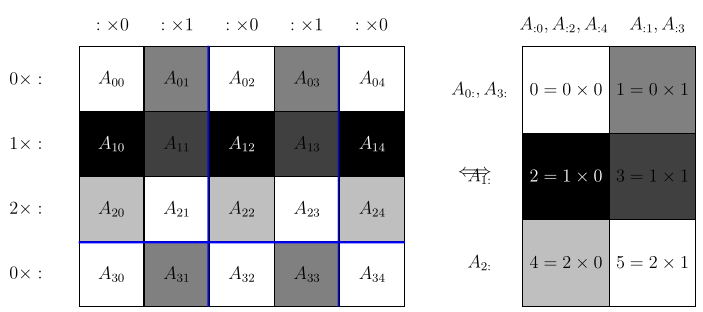
\includegraphics[width=0.8\textwidth]{src/2dbc.png}
        \caption{A split matrix distributed on nodes $\Leftrightarrow$ the grid of nodes and their affected column/row combination of blocks}
        \label{fig:2dbc}
\end{figure}


The goal of this project is to implement three variations of a distributed GEMM algorithm using different MPI communication strategies and then benchmark their performance across a range of problem sizes and node configurations.

\subsection{Blocking peer-to-peer communications}

This variant uses \texttt{MPI\_Ssend} and \texttt{MPI\_Recv} to transmit required blocks between processes.
Each node sends the blocks it owns to other nodes in its row (for \(A\)) or column (for \(B\)), then performs local computation.
Communication and computation are strictly serialized. \\

Using VITE, we can visualize the blocking peer-to-peer communication pattern for GEMM.
We set the number of nodes to \(p = q = 2\), the matrix size to \(m = n = k = 10\) and the number of blocks per node to \(b = 5\).
\begin{figure}[H]
    \centering
    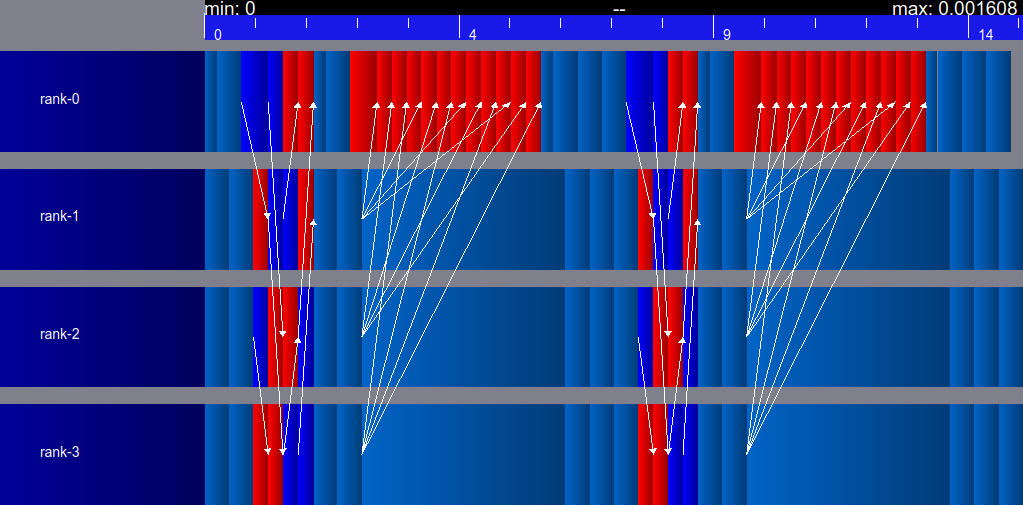
\includegraphics[width=0.8\textwidth]{src/p2p.png}
    \caption{Blocking peer-to-peer communication for GEMM}
    \label{fig:p2p}
\end{figure}

Clear vertical barriers appear where all processes must wait for communication to complete before proceeding to computation.
Some processes finish their communication earlier but must wait for others, leading to inefficient resource utilization.


\subsection{Blocking collective communications}

Here, \texttt{MPI\_Bcast} is used instead of multiple individual sends.
A node that owns a block of \(A\) or \(B\) broadcasts it to all nodes in the same row or column communicator.
This reduces the number of messages and synchronizes communication across each dimension.\\

Using VITE, we can visualize the blocking collective communication pattern for GEMM in the same configuration as before.
\begin{figure}[H]
    \centering
    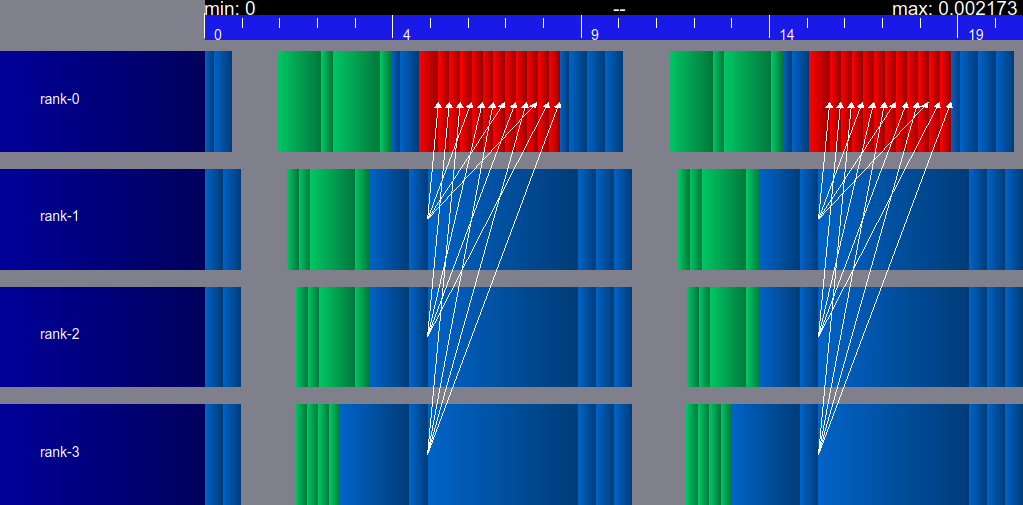
\includegraphics[width=0.8\textwidth]{src/bcast.png}
    \caption{Blocking collective communication for GEMM}
    \label{fig:bcast}
\end{figure}

\texttt{MPI\_Bcast} reduces the number of individual messages by leveraging optimized collective communication trees.


\subsection{Non-blocking peer-to-peer communications}

This approach uses \texttt{MPI\_Irecv}, \texttt{MPI\_Issend}, and \texttt{MPI\_Wait} to overlap communication with computation.
Nodes post non-blocking receives and sends in advance (controlled by a lookahead parameter), allowing them to proceed with computation while communication is ongoing. \\

Using VITE, we can visualize the non-blocking peer-to-peer communication pattern for GEMM in the same configuration as before.
\begin{figure}[H]
    \centering
    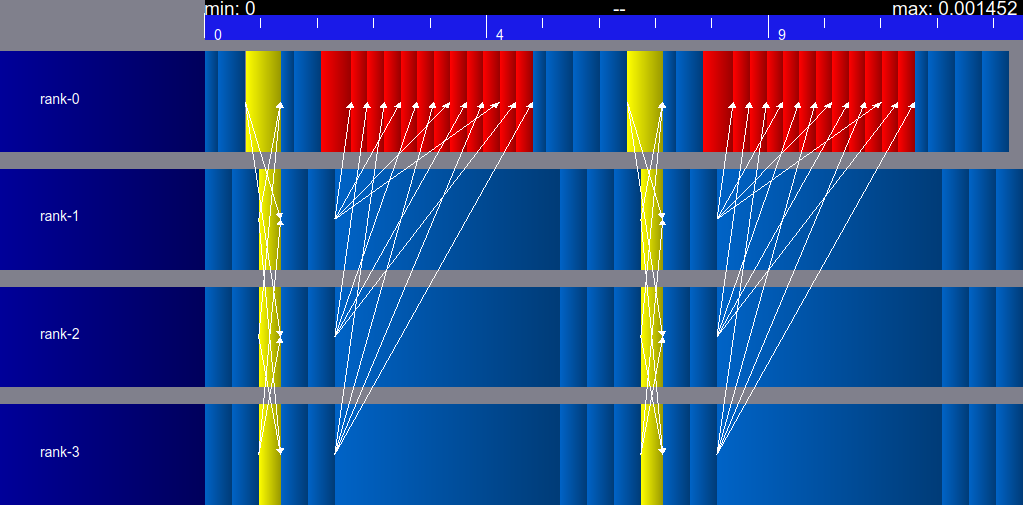
\includegraphics[width=0.8\textwidth]{src/p2p-i-la.png}
    \caption{Non-blocking peer-to-peer communication for GEMM}
    \label{fig:p2p_i_la}
\end{figure}

Communication and computation phases overlap significantly, reducing total execution time.



\section{Benchmarking}

To evaluate the performance of our implementations, we conducted a series of benchmarks.
All benchmarks were performed using SimGrid, a simulation framework for MPI programs.
Each experiment was repeated 5 times, and performance values were collected from the trace outputs. \\
For each simulation run, we tried different \texttt{lookahead} values for the non-blocking peer-to-peer implementation.
The following results show the best performance achieved for each configuration.

\subsection{Raw performance}

We evaluated the raw performance of each implementation by measuring the number of Gflop/s achieved for different matrix sizes (\(m = n = k\)) on a fixed grid (\(p = q = 2\)).

\begin{figure}[H]
    \centering
    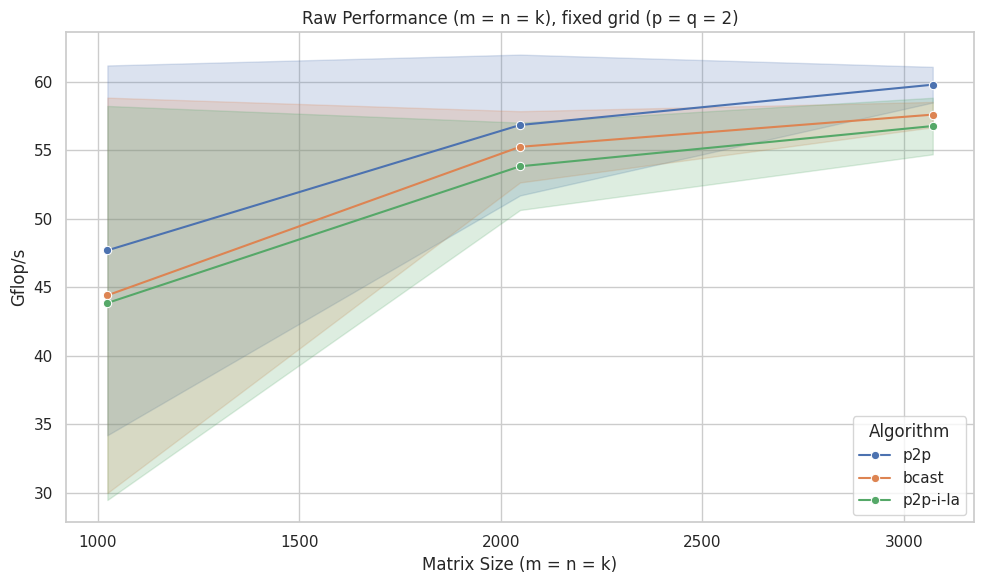
\includegraphics[width=0.8\textwidth]{src/raw_performance.png}
    \caption{Raw performance of the three implementations for different matrix sizes.}
    \label{fig:raw_performance}        
\end{figure}

Blocking peer-to-peer (p2p) consistently outperforms both blocking variants.
All implementations show increasing performance with larger matrix sizes, indicating better computational-to-communication ratios.


\subsection{Strong scaling}

We evaluated strong scaling by fixing the problem size (\(m = n = k = 2048\)) and varying the number of nodes (\(p \times q\)).

\begin{figure}[H]
    \centering
    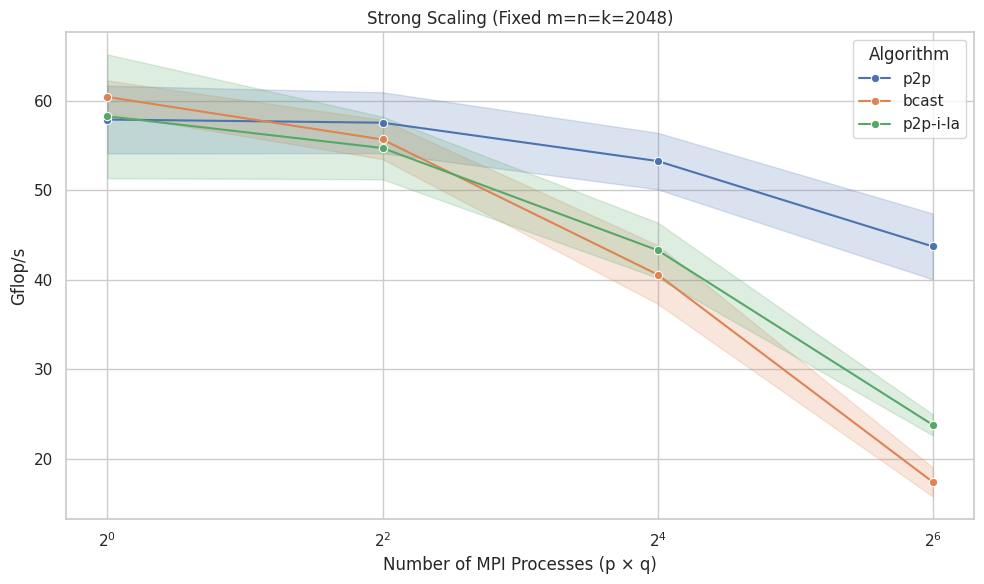
\includegraphics[width=0.8\textwidth]{src/strong_scaling.png}
    \caption{Strong scaling performance of the three implementations for a fixed problem size.}
    \label{fig:strong_scaling}     
\end{figure}

All implementations show declining efficiency with increasing process count, indicating parallel overhead.
The fixed problem size means each process has less work, making communication overhead more prominent.


\subsection{Weak scaling}

We evaluated weak scaling by increasing both the problem size and the number of nodes proportionally.

\begin{figure}[H]
    \centering
    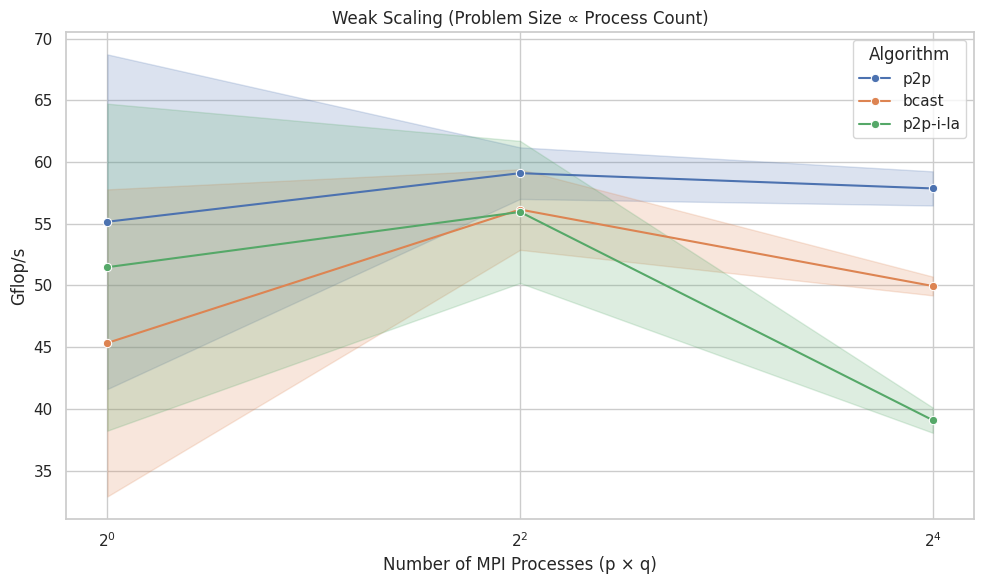
\includegraphics[width=0.8\textwidth]{src/weak_scaling.png}
    \caption{Weak scaling performance of the three implementations for increasing problem size and number of nodes.}
    \label{fig:weak_scaling}
\end{figure}

Weak scaling should maintain constant performance as both work and resources increase proportionally.
However, we observe that only the blocking peer-to-peer (p2p) implementation remains constant, while the other two implementations show decreasing performance.



\section{Conclusion}

Our benchmarking study of three distributed GEMM implementations reveals several important findings about MPI communication strategies in parallel matrix multiplication.
The blocking peer-to-peer implementation consistently demonstrated the best performance across all tested scenarios, achieving a better scaling overall.
Surprisingly, the non-blocking peer-to-peer implementation and the collective broadcast approach showed inferior performance compared to the basic blocking implementation, which contradicts theoretical expectations and common parallel computing wisdom that communication-computation overlap should provide performance benefits.



\end{document}